\documentclass[a4paper,12pt]{article}

\usepackage[utf8]{inputenc}
\usepackage[T1]{fontenc}
\usepackage[brazil]{babel}
\usepackage{graphicx}
\usepackage{xcolor}
\usepackage{tcolorbox}
\usepackage{geometry}
\usepackage{tikz}
\usetikzlibrary{positioning, shapes.multipart}
\geometry{margin=2.5cm}
 
\definecolor{meuazul}{RGB}{0, 79, 151}

\begin{document}

\begin{center}
    
\includegraphics[width=3cm]{logo.png} \\
    \vspace{0.5cm}
    \textbf{\large Engenharia da Qualidade e Confiabilidade} \\
    \textbf{Atividade Prática: Planning Poker}
\end{center}

\vspace{1cm}

\begin{tcolorbox}[colback=meuazul!5, colframe=meuazul, title=\textbf{HU002: Gerenciamento de Veterinários}]
    
    \textbf{Título:} Cadastro e Gestão de Profissionais Veterinários
    
    \vspace{0.3cm}
    \textbf{Descrição (História de Usuário):} \\
    Como \textbf{Administrador da Fazenda}, \\
    quero \textbf{cadastrar, visualizar, atualizar e remover veterinários}, \\
    para \textbf{manter um registro dos profissionais habilitados a atender os animais e registrar suas intervenções}.
    
    \vspace{0.3cm}
    \textbf{Valor de Negócio:} \\
    Garante a rastreabilidade técnica dos atendimentos e facilita o contato com especialistas.
    
    \vspace{0.3cm}
    \textbf{Prioridade:} Média
    
\end{tcolorbox}

\vspace{0.5cm}

\section*{Story Points e Protótipos de Tela}
\begin{enumerate}
    \item \textbf{Cadastrar Veterinário:} Inserir CRMV (ID único), Nome, Especialidade e Telefone.
    \begin{itemize}
        \item \textit{Explicação:} Tela para registro de novos profissionais. O CRMV deve ser validado para garantir que o cadastro é único.
        \begin{center} 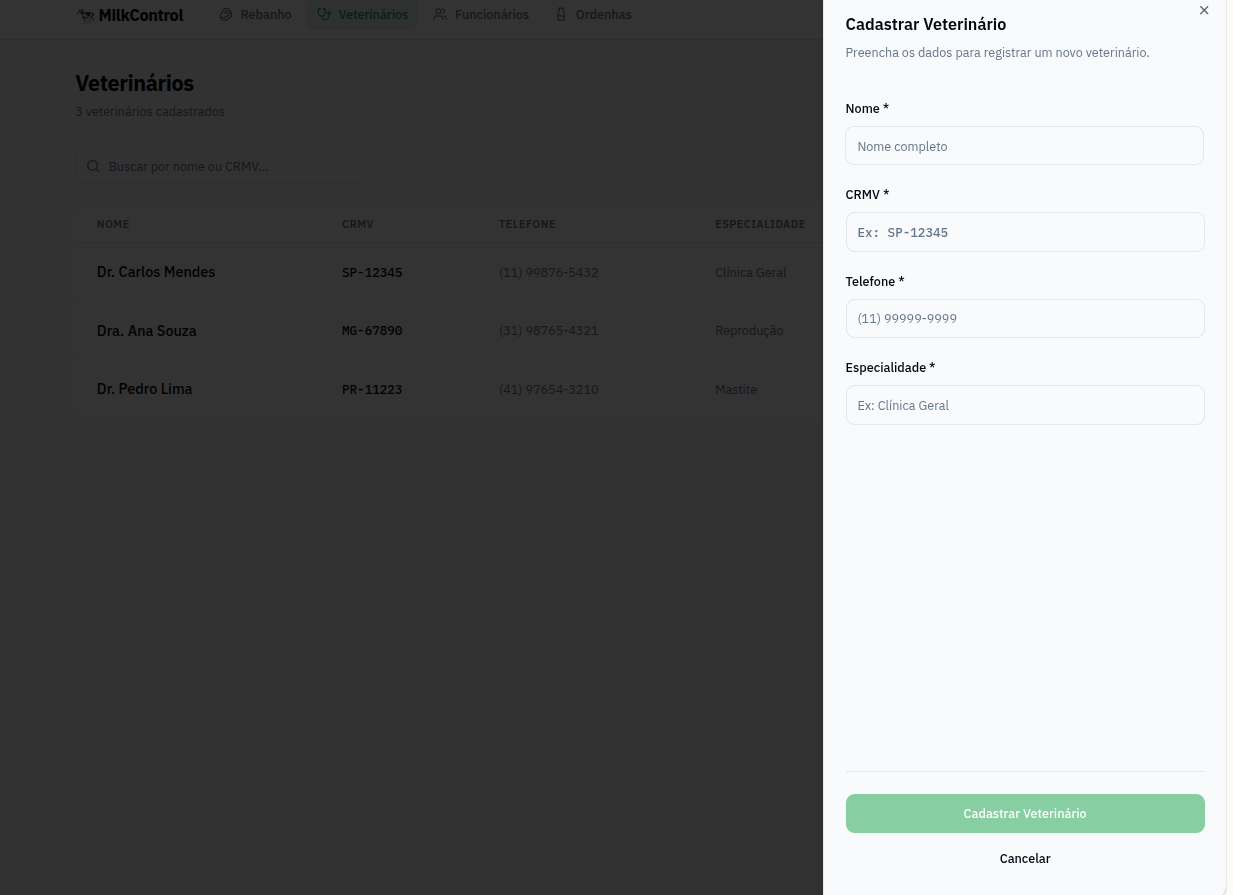
\includegraphics[width=0.7\textwidth]{create_vet.png} \end{center}
    \end{itemize}

    \item \textbf{Visualizar Lista:} Listagem de todos os veterinários com filtros por especialidade.
    \begin{itemize}
        \item \textit{Explicação:} Permite encontrar rapidamente um profissional específico em caso de emergência ou rotina sanitária.
        \begin{center} 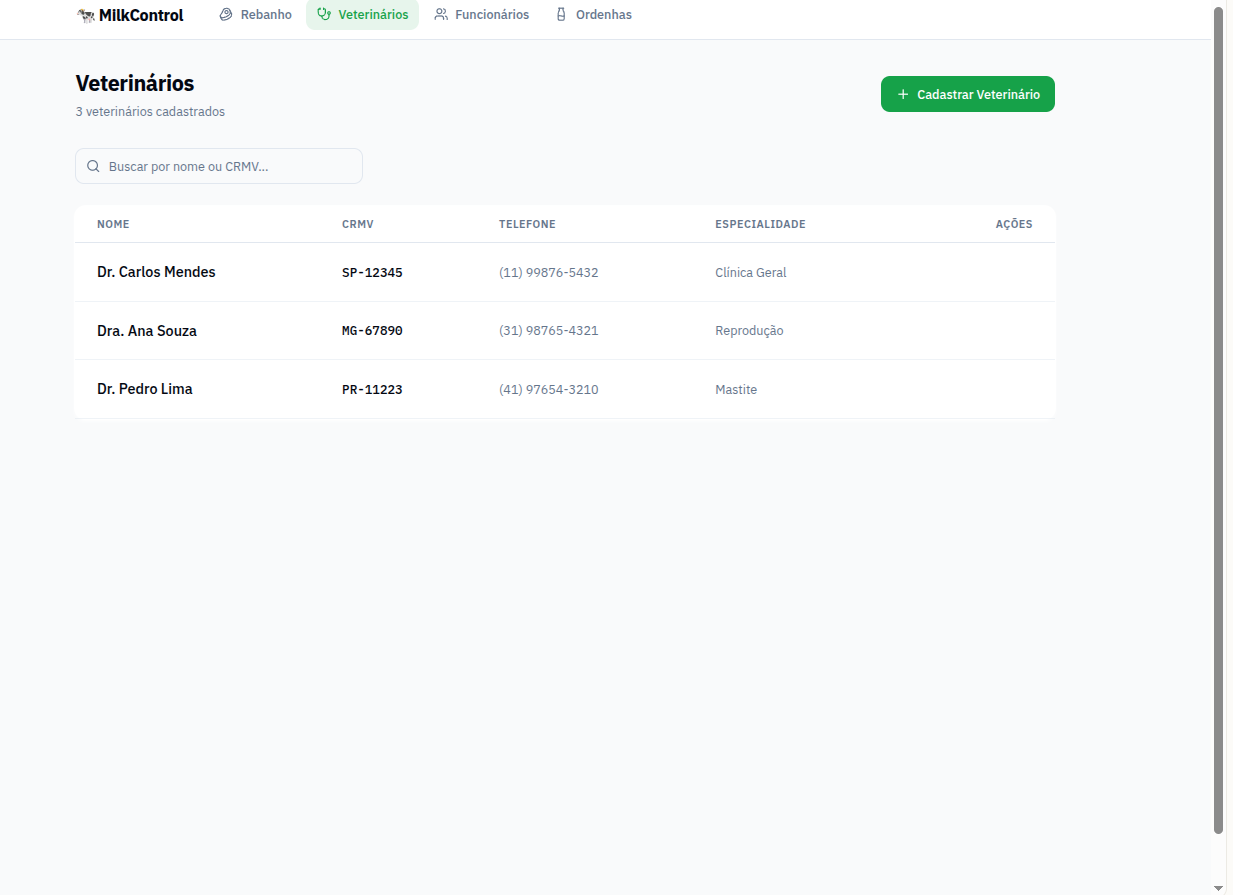
\includegraphics[width=0.7\textwidth]{show_vet.png} \end{center}
    \end{itemize}

    \item \textbf{Atualizar Dados:} Edição de dados de contato e especialização.
    \begin{itemize}
        \item \textit{Explicação:} Mantém os dados de contato do profissional sempre atualizados no sistema.
        \begin{center} 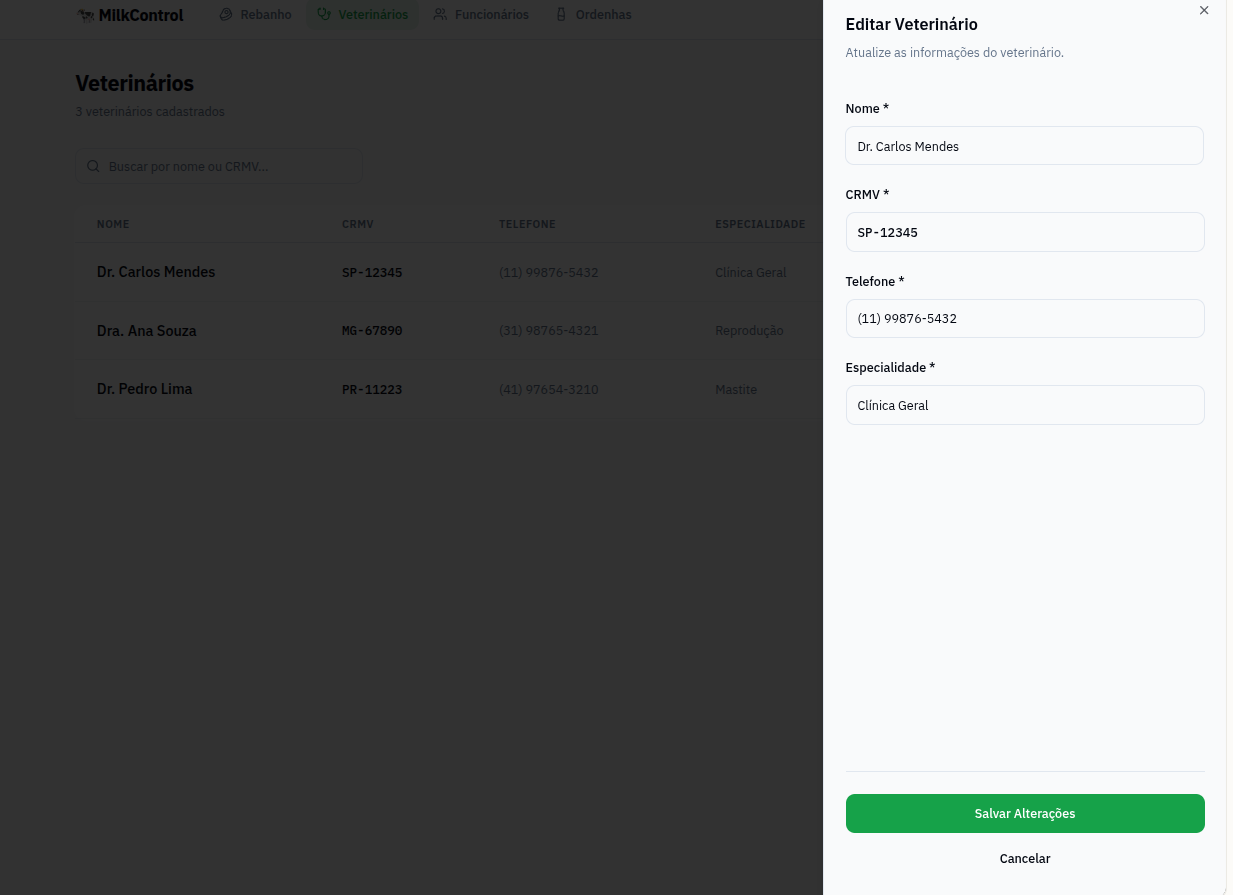
\includegraphics[width=0.7\textwidth]{edit_vet.png} \end{center}
    \end{itemize}

    \item \textbf{Excluir Registro:} Remoção do profissional do sistema.
    \begin{itemize}
        \item \textit{Explicação:} Permite remover profissionais que não prestam mais serviços, com validação para não apagar históricos de atendimento obrigatórios.
        \begin{center} 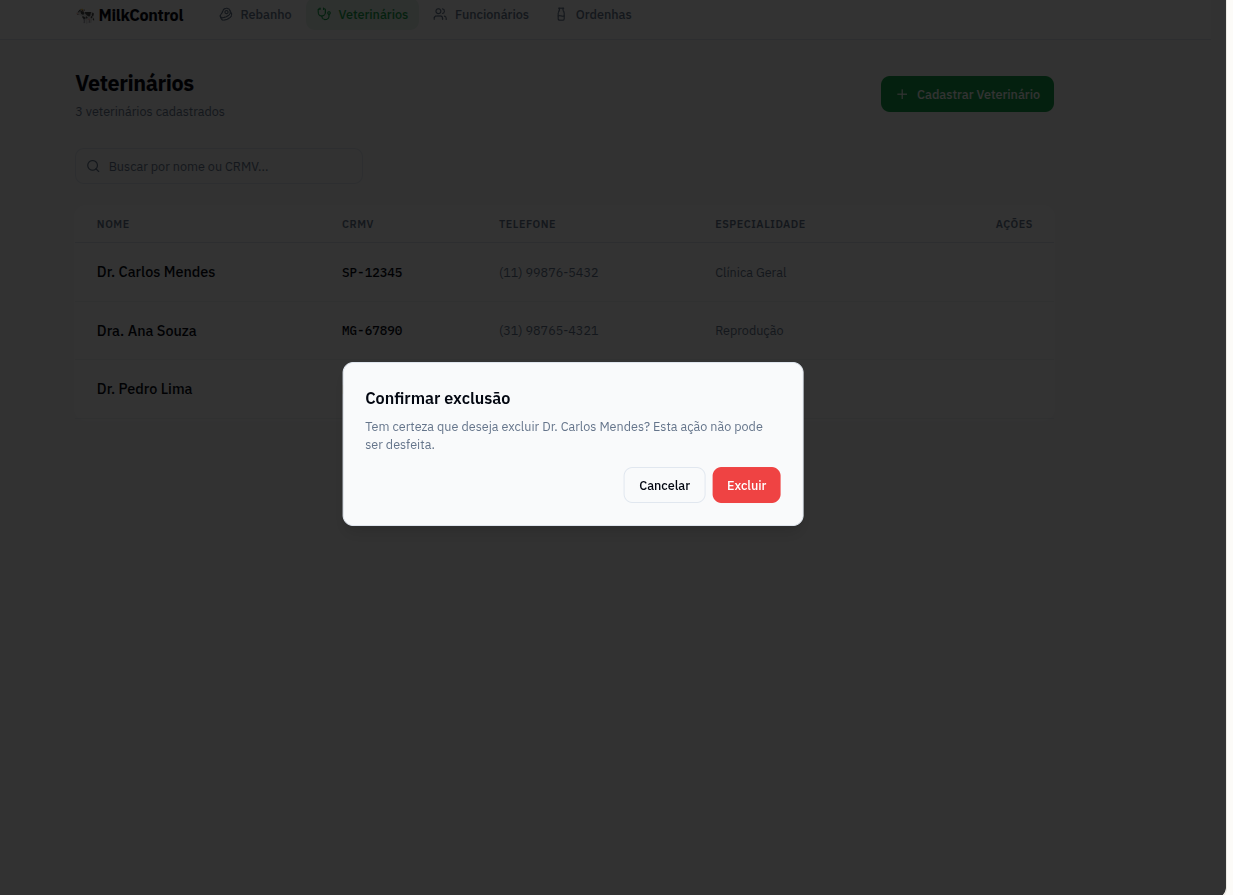
\includegraphics[width=0.7\textwidth]{delete_vet.png} \end{center}
    \end{itemize}
\end{enumerate}

\vspace{0.5cm}

\section*{Modelo de Dados (Diagrama de Classes)}

\begin{center}
\begin{tikzpicture}[
    node distance=2cm,
    classBox/.style={
        draw=meuazul,
        thick,
        fill=white,
        minimum width=4cm,
        rectangle split,
        rectangle split parts=3,
        align=left,
        rounded corners=2pt
    }
]

% Classe Veterinario
\node[classBox] (Vet) {
    \textbf{Veterinario}
    \nodepart{second}
    - crmv: String \{PK\} \\
    - nome: String \\
    - especialidade: String \\
    - telefone: String
    \nodepart{third}
    + realizarAtendimento()
};

% Classe Vaca
\node[classBox, right=3.5cm of Vet] (Vaca) {
    \textbf{Vaca}
    \nodepart{second}
    - brinco: String \{PK\} \\
    - nome: String \\
    - raca: String
    \nodepart{third}
};

% Associação
\draw[thick, meuazul] (Vet) -- (Vaca) 
    node[pos=0, above right] {1} 
    node[pos=1, above left] {*};

\end{tikzpicture}
\end{center}

\vspace{0.5cm}

\section*{Atividade: Estimativa com Planning Poker}

Cada grupo deverá estimar o esforço das funcionalidades utilizando \textbf{Story Points} (Fibonacci):

\begin{center}
\textbf{0, 1, 2, 3, 5, 8, 13, 21}
\end{center}

\vspace{1cm}

\begin{center}
    \rule{0.5\textwidth}{0.4pt} \\
    \small UniRV - Engenharia de Software
\end{center}

\end{document}
